% Generated from paper_v6.md; original Markdown is unchanged.
\documentclass{article}
% Anonymous workshop submission. Do not use final or preprint for review.
\PassOptionsToPackage{numbers,sort&compress}{natbib}
\usepackage[dblblindworkshop]{neurips_2026}
\workshoptitle{Physical World AI: Geometry, Characteristics, and Multimodal Sensing}
\usepackage[T1]{fontenc}
\usepackage{amsmath,amssymb}
\usepackage{graphicx,booktabs,longtable,array,calc}
\usepackage{microtype,xcolor,newunicodechar}
\usepackage{url}
\usepackage[hidelinks,unicode]{hyperref}
\newunicodechar{−}{\ensuremath{-}}
\newunicodechar{±}{\ensuremath{\pm}}
\newunicodechar{×}{\ensuremath{\times}}
\newunicodechar{Δ}{\ensuremath{\Delta}}
\newunicodechar{θ}{\ensuremath{\theta}}
\newunicodechar{φ}{\ensuremath{\phi}}
\newunicodechar{ε}{\ensuremath{\epsilon}}
\newunicodechar{→}{\ensuremath{\rightarrow}}
\newunicodechar{≤}{\ensuremath{\leq}}
\newunicodechar{≥}{\ensuremath{\geq}}
\providecommand{\tightlist}{\setlength{\itemsep}{0pt}\setlength{\parskip}{0pt}}
\providecommand{\pandocbounded}[1]{#1}
\setlength{\emergencystretch}{2em}
\graphicspath{{figures/}{../figures/}}
\hypersetup{pdftitle={Feature Prediction and Gait Laterality: A Geometry Audit of Skeleton JEPA},pdfauthor={Anonymous Author(s)},pdfcreator={LaTeX},pdfsubject={Physical World AI workshop submission}}
\title{Feature Prediction and Gait Laterality: A Geometry Audit of Skeleton JEPA}
\author{Anonymous Author(s)}
\begin{document}
\maketitle
\begin{abstract}
Human movement provides a useful test of whether predictive representations preserve the geometry of an articulated body. Left--right reflection supplies a known transformation, while differences between the two sides provide an observable quantity whose sign should change under that transformation. We study this relationship in a skeleton Joint-Embedding Predictive Architecture using pose sequences from gait videos. A source-separated evaluation compares trained and initial encoders, tests reflection behavior, and changes the anatomical and temporal placement of hidden training targets. The available experiments show that predicting a clip's hidden features more accurately than another clip's features can coexist with weaker recovery of a signed movement contrast. Motion-sensitive summaries improve the initial-encoder readout, while motion-weighted and connected-region masks provide no demonstrated advantage over their matched random references. We distinguish this evidence from exact symmetry imposed at the output and from synthetic demonstrations of explicit reflection training. The study contributes an evaluation of articulated-body representations for Physical World AI, identifying a gap between feature prediction and the recovery of a coordinate-derived movement contrast.
\end{abstract}
\section{Introduction}\label{introduction}

Walking provides a useful setting for studying predictive representations because an articulated body combines anatomical regularity with movement that can differ between its sides. Exchanging left and right preserves some quantities, such as total movement, while reversing a signed left-minus-right contrast. A useful representation should retain the information needed for the intended measurement while responding predictably to changes of coordinates.

This distinction has a concrete health motivation. Post-stroke gait can exhibit spatial or temporal asymmetry, Parkinson's research examines unequal arm swing, and cerebral palsy includes unilateral and bilateral presentations. Muscular disorders can also change pelvic and limb coordination. These clinical observations motivate examining bilateral structure without making a signed speed contrast a general measure of health. Post-stroke gait~\citep{ref01}, arm-swing study~\citep{ref02}, cerebral-palsy gait study~\citep{ref03}, muscular-dystrophy kinematics~\citep{ref04}

We study a skeleton Joint-Embedding Predictive Architecture, or JEPA: an encoder and predictor learn to estimate hidden features using the remaining observations, while a slowly updated encoder supplies their targets. Our initial null is that this pretraining provides no gain over matched initial weights in recovering a signed movement contrast on excluded source videos. Further comparisons ask whether changing the anatomy, motion content or temporal arrangement of hidden targets produces such a gain.

The resulting investigation connects a known coordinate transformation, a target with a defined sign response, and a paired training comparison. We first examine the measurement and reflection rules, then test whether anatomically motivated training changes improve its recovery, and finally compare the predictor's feature correspondence with the frozen encoder's usefulness. The sequence is a retrospective account of development; it does not imply that all later questions were preregistered together.

The workshop contribution concerns evaluation of articulated-body representations. Its main evidence is that successful correct-clip feature prediction coexists with poorer laterality readouts after pretraining. The study has no demonstrated real-data forecasting or multimodal-fusion result. Those boundaries matter when considering this representation as a component of a physical world model.

\section{Context in predictive and geometric learning}\label{context-in-predictive-and-geometric-learning}

S-JEPA~\citep{ref05} establishes skeleton latent prediction, and MAMP~\citep{ref06} motivates motion-informed masking. The recent SLiM preprint~\citep{ref07} includes connected anatomical masks. Our MAMP-style arm adapts its official-code sampler while retaining the JEPA feature target; it does not reproduce the full MAMP method.

seq-JEPA~\citep{ref08} studies invariant and equivariant representations, while Soft Equivariance Regularization~\citep{ref09} examines geometric supervision and its tradeoffs. These precedents motivate evaluating geometric agreement together with observable utility.

Recent V-JEPA 2.1~\citep{ref10} and Human-JEPA~\citep{ref11} preprints investigate dense supervision and human-focused anticipation, respectively; GaitJEPA~\citep{ref12} already applies predictive learning to gait silhouettes. The novelty here is the controlled evaluation of a side-sensitive coordinate target, rather than the combination of gait and JEPA or the invention of anatomical masking.

\section{Measurement, training and evaluation}\label{measurement-training-and-evaluation}

\subsection{Cohort and target}\label{cohort-and-target}

The local GAVD~\citep{ref13} inventory contains 666 annotations and 642 matching pose archives. Quality control retains 625 clips from 93 source videos. Its categories are normal, Parkinson's, stroke, myopathic and cerebral-palsy gait. They stratify source assignments and describe the dataset; they supply no encoder supervision. The category census and clinical interpretation limits appear in Appendix E.

Coordinates use image-normalized horizontal and vertical positions and inferred depth scaled relative to crop width. Their Euclidean differences are coordinate-derived movement measures, not calibrated metric three-dimensional speeds. Aspect ratio, projection, detector error and visibility can affect them.

For each of five bilateral pairs---shoulders, knees, ankles, heels, and foot tips---we calculate left and right speeds using observed timestamps and only transitions for which both landmarks are observed at both ends. Let their median speeds be \(m_{L,k}\) and \(m_{R,k}\). The target is

\[
y(x)=\frac{1}{5}\sum_{k=1}^{5}
\frac{m_{L,k}-m_{R,k}}{m_{L,k}+m_{R,k}+\epsilon}.
\]

All five pairs must provide at least eight shared valid transitions. Hips establish the pelvis reference but are excluded from this target: pelvis centering makes their speed magnitudes identical. The target is calculated before input interpolation and resizing. It measures asymmetry of median coordinate speed, not stride duration, phase coordination, or limb loading. Oppositely signed pair contrasts can cancel in the average. Similarly, left- and right-affected people could have substantial individual asymmetry but a near-zero group-average signed target. A small \(y\) therefore does not establish healthy or bilaterally symmetric gait.

Reflection \(M\) negates the centered horizontal coordinate and exchanges all anatomically paired landmarks, together with validity. Consequently, \(M^2x=x\) and \(y(Mx)=-y(x)\). This identity is a property of the coordinate operation and formula, rather than evidence that every reflected recording would occur naturally.

\subsection{Preservation and information boundaries}\label{preservation-and-information-boundaries}

The encoder input is prepared separately. Visibility at least 0.45 and finite coordinates determine observations; up to four missing samples can be interpolated for input only. Pelvis normalization removes translation and applies a body scale. Resizing then samples 64 locations along normalized sequence index, without preserving the original timestamp intervals. Values under invalid entries are zero-filled only alongside an explicit validity mask.

\begin{table}[htbp]
\centering
\small
\begin{tabular}{@{}
  >{\raggedright\arraybackslash}p{(\linewidth - 4\tabcolsep) * \real{0.1800}}
  >{\raggedright\arraybackslash}p{(\linewidth - 4\tabcolsep) * \real{0.2600}}
  >{\raggedright\arraybackslash}p{(\linewidth - 4\tabcolsep) * \real{0.5600}}@{}}
\toprule\noalign{}
\begin{minipage}[b]{\linewidth}\raggedright
Stage
\end{minipage} & \begin{minipage}[b]{\linewidth}\raggedright
Array shape
\end{minipage} & \begin{minipage}[b]{\linewidth}\raggedright
What remains associated; what changes
\end{minipage} \\
\midrule\noalign{}

Archived clip & \(T_i\times33\times4\), plus frame numbers and frame rate & Coordinate channels and visibility remain linked to one source and sequence. \\
Target branch & \(T_i\times33\times3\), validity \(T_i\times33\) & Original timestamps and observed-only paired transitions determine the target. \\
Model input & \(64\times33\times3\), validity \(64\times33\) & Joint identities remain; interpolation, normalization and resampling alter coordinate values and timing. \\
Four-frame patches & \(16\times33\times12\) & Each patch concatenates four three-coordinate observations of one landmark; complete validity determines eligibility. \\
Embedded token grid & \(16\times33\times96\) & Time-block and landmark indices identify each 96-dimensional feature. \\
Batch with mask & \(B\times528\times96\), plus target indices and validity & The full grid remains allocated. Target selection and validity determine loss contributions; paired arms match counts per clip. \\
\bottomrule
\end{tabular}
\end{table}

The pipeline preserves the correspondence between recordings, landmarks, masks, and targets. It cannot promise preservation of the exact observed shape or speed after preparation. Cohort preparation occurs before split-file creation in the implementation; it uses deterministic clip-local operations rather than statistics fitted across sources. Source membership is fixed before training sampling, augmentation, and model fitting.

\subsection{Where laterality enters training}\label{where-laterality-enters-training}

\begin{figure}[!tbp]
\centering
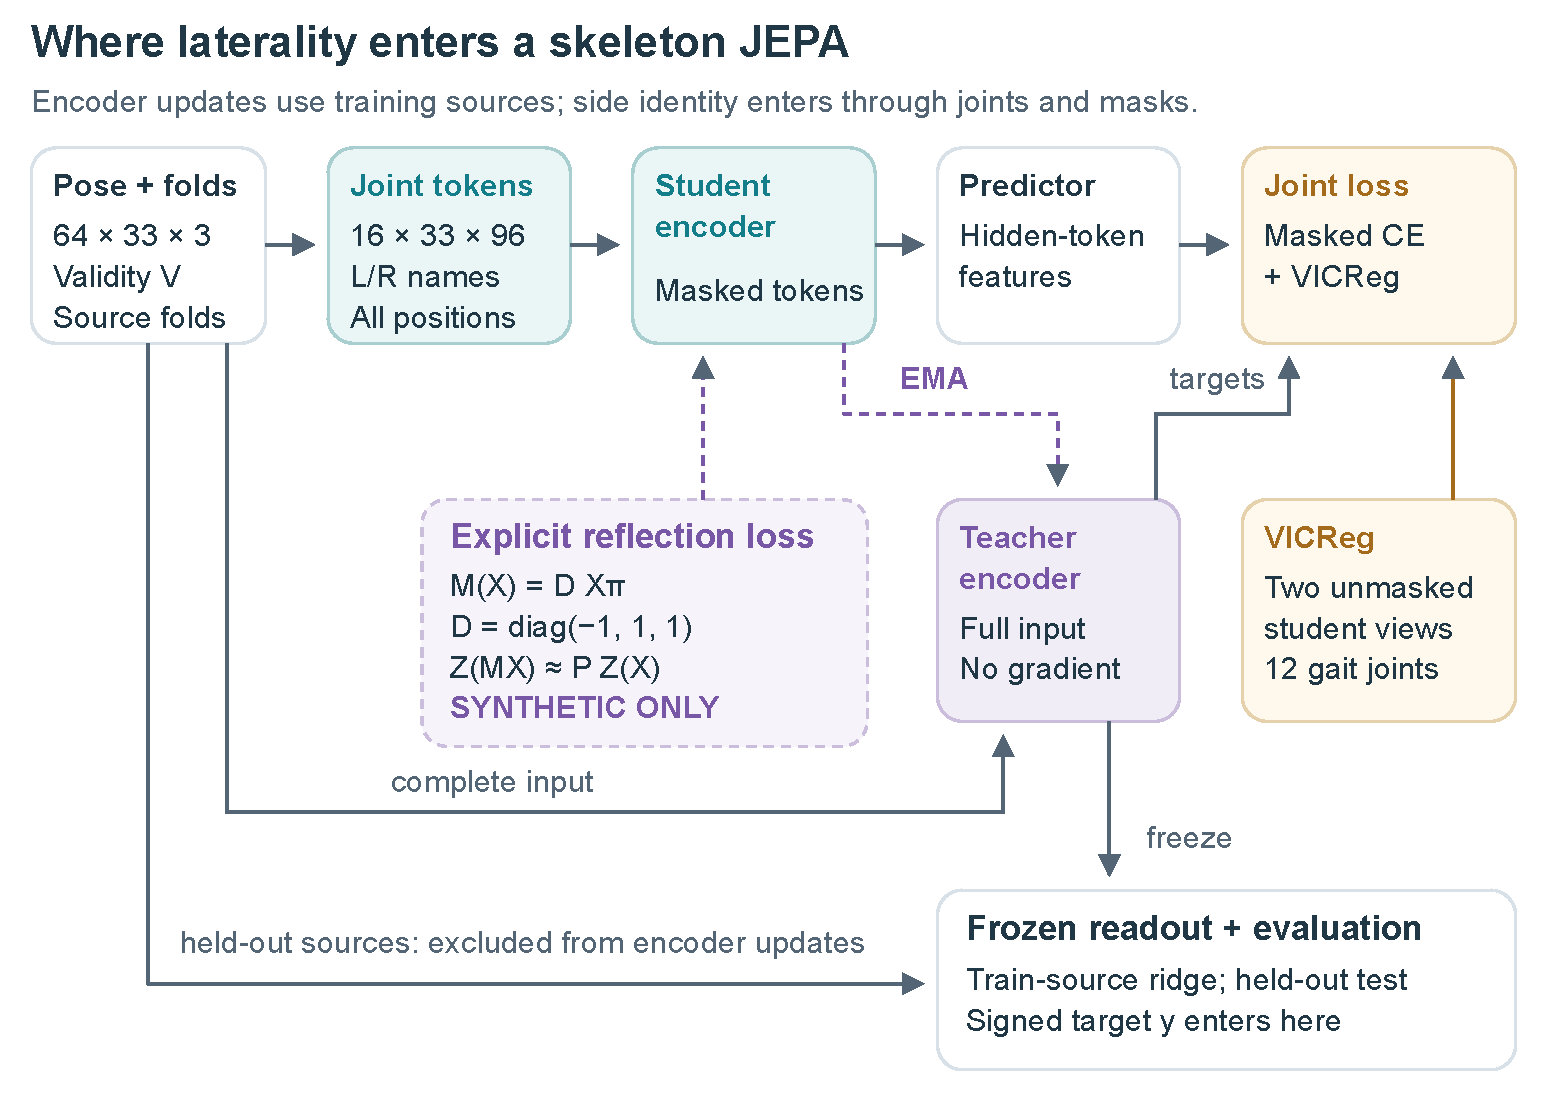
\includegraphics[width=\linewidth]{training_pipeline_compact_print.pdf}
\caption{Anatomical identities and gait-based masking or pooling introduce laterality into the completed representation-learning recipe. The dotted branch adds an explicit token-reflection penalty to the online encoder and has synthetic evidence only. The signed target is used after pretraining by the frozen-feature readout. Clip-local preparation precedes source-fold creation in the code; every subsequent training draw and transformed view inherits the source assignment. The expanded pipeline (Figure~\ref{fig:training_pipeline}) details the shapes and gradient paths.}\label{fig:training_pipeline_compact}
\end{figure}

Five outer folds hold out 19, 19, 19, 18 and 18 sources, containing 189, 182, 72, 77 and 105 clips. All clips, mirrors and augmentations from a video remain together. Each fold and seed starts a new encoder using only its outer-training sources; source-balanced sampling controls the contribution of videos with many clips. Four inner folds in the original audit and three in the extensions select ridge readout penalties. Each imputer and scaler is fitted within the corresponding inner fitting partition, then refitted with the selected penalty on all outer-training sources. Inner validation selects the readout only: its unlabeled clips already entered that outer fold's encoder pretraining.

All completed real-data comparisons use 64 frames and 33 landmarks, width 96, encoder/predictor depths 4/2, four attention heads, batch size 20, and 1,200 updates. The online encoder retains the full token grid but zeros hidden coordinate embeddings before adding positions. The predictor estimates teacher distributions at hidden locations using cross-entropy. The teacher receives no gradients and follows an exponential moving average of online weights. An auxiliary VICReg loss, weighted by 0.05, regularizes agreement and feature variation over two unmasked geometric views pooled at twelve gait landmarks. Thus changing hidden-target eligibility does not remove all anatomical priors.

Paired arms share initialization, source draws, geometric views and update counts, with separate random streams for masking. Mask losses preserve each clip's own target indices; the latest variable-count implementation averages within clip before averaging clips. Invalid targets do not contribute. The regularizer legitimately receives complete training views, so the masked prediction pathway is not the encoder's only exposure to those observations.

The original reflection variant mirrors training clips with probability 0.5. The latest motion/region grid uses neither reflection augmentation nor an explicit reflection penalty. Notebook 09 implements the latter through two original/reflected online-encoder passes, aligning anatomical tokens while leaving feature channels unchanged. Its executed example is synthetic; Appendix F gives its loss and additional compute. None of these encoder objectives uses the signed target or an affected-side label.

\subsection{Evaluation and statistical inference}\label{evaluation-and-statistical-inference}

For \(V\) sources and \(n_v\) clips from source \(v\), each clip has weight \(w_{vi}=1/(Vn_v)\). With \(\bar y_w=\sum w_{vi}y_{vi}\), \[
R^2_w=1-\frac{\sum_{vi}w_{vi}(y_{vi}-\hat y_{vi})^2}
{\sum_{vi}w_{vi}(y_{vi}-\bar y_w)^2}.
\] Each source therefore receives equal total weight even when it supplies many clips. Within a seed, predictions from all five held-out folds are pooled before computing \(R^2\); the reported result averages the five seed-specific scores. It is neither an average of fold \(R^2\) values nor a score from an ensemble of seed-averaged predictions. Negative \(R^2\) means squared error exceeds variation around the weighted evaluation mean; a separately fitted training-source mean is the usable prediction baseline.

Paired uncertainty resamples entire videos while retaining their clips and paired seed predictions. For a mask comparison the null is no positive difference in source-balanced readout performance relative to the count-matched random policy; for learning it is no positive difference relative to matched initialization. These are superiority questions, and no equivalence margin or power guarantee is established. The latest mask contrasts and this revision's learning contrasts use 2,000 resamples. Their intervals condition on the fitted models and exclude full-retraining and new-split uncertainty. The historical original summary records a separate 2,000-resample analysis, whose complete inputs remain unavailable. Repeated seeds and diagnostic mask draws are not independent participants. Subsequent experiments were informed by the same development cohort, so their source separation does not make the overall research trajectory an untouched confirmatory study.

\section{Results as a sequence of tests}\label{results-as-a-sequence-of-tests}

\subsection{Measurement agreement and the original reflection question}\label{measurement-agreement-and-the-original-reflection-question}

Recomputing the target on prepared input provides finite paired measurements for 623 clips from 92 sources. The source-weighted sign agreement with the original measurement is 70.4\%, and direct calculation-agreement \(R^2\) is 0.218. This newly repeated descriptive diagnostic flags a mismatch in the measurement path. It neither localizes the responsible preparation step nor estimates a model's accuracy or information ceiling.

The historical reflection audit reports no demonstrated trained-over-initial predictive gain. Its documentation also records a small improvement in the specified token discrepancy with reflection augmentation: augmented-minus-vanilla \(q=-0.00843\), interval \([-0.01020,-0.00687]\). Prediction does not show a corresponding demonstrated improvement. Both trained variants remain worse than their initialization under that token action. This geometric success is therefore limited to one measured criterion.

The original reports and predictions are absent from this checkout, while rounded figure values and a more precise historical README ledger remain. We use them as historical context, with the exact available values and their provenance in Appendix G. Their full uncertainty analysis was not repeated here. The direct test fixes the channel action to identity; failure does not rule out another learned reflection transformation. Likewise, an algebraically odd output or constant nonzero token vector can satisfy a symmetry criterion without useful movement prediction.

\subsection{Do different hidden targets improve the observable outcome?}\label{do-different-hidden-targets-improve-the-observable-outcome}

Notebook 12's retained summary compares gait-only and all-landmark scattered targets at matched counts and finds no demonstrated advantage. Its raw prediction directory is also absent locally, so its numerical results remain supporting context. The main evidence comes from the complete Notebook 18 grid: 50 paired fold/seed jobs, containing 125 encoders across motion and region comparisons.

The latest motion budget uses 0.5 of the smaller gait-derived pool, yielding an average of 80.771 targets, about 17\% of valid all-landmark tokens. It does not hide half the body grid. MAMP-style and robust motion weighting increase target-motion enrichment under the common audit statistic. Connected regions hide about 9.9\% of valid tokens, reducing immediate visible time brackets from 0.699 to zero and visible anatomical neighbors from 0.988 to 0.512. These are successful changes to selection and local context; they do not establish what the contextualized teacher features represent.

\begin{table}[htbp]
\centering
\small
\begin{tabular}{@{}
  >{\raggedright\arraybackslash}p{(\linewidth - 4\tabcolsep) * \real{0.4600}}
  >{\raggedleft\arraybackslash}p{(\linewidth - 4\tabcolsep) * \real{0.2200}}
  >{\raggedright\arraybackslash}p{(\linewidth - 4\tabcolsep) * \real{0.3200}}@{}}
\toprule\noalign{}
\begin{minipage}[b]{\linewidth}\raggedright
Alternative minus its own random reference
\end{minipage} & \begin{minipage}[b]{\linewidth}\raggedleft
\(\Delta R^2\)
\end{minipage} & \begin{minipage}[b]{\linewidth}\raggedright
95\% source interval
\end{minipage} \\
\midrule\noalign{}

MAMP-style motion weighting & −0.0008 & {[}−0.0204, 0.0153{]} \\
Robust motion mixture & 0.0005 & {[}−0.0155, 0.0152{]} \\
Connected region & −0.0087 & {[}−0.0333, 0.0177{]} \\
\bottomrule
\end{tabular}
\end{table}

Each comparison covers 625 clips, 93 sources and five seeds. Motion and region families have different budgets and separate references. Their intervals allow small improvements or losses, establishing neither superiority nor equivalence. Whole trajectories and interior gaps have coverage audits but no completed training comparison. No mask is selected as best on these outer-test results.

\subsection{Does pretraining help when the readout retains more movement statistics?}\label{does-pretraining-help-when-the-readout-retains-more-movement-statistics}

A mean summary combines left-minus-right and left-plus-right feature means for five pairs, giving 960 features. Adding temporal standard deviations, mean absolute feature increments and ten support fractions gives 2,890. The latter improves the initial encoder from \(R^2=0.0708\) to \(0.2225\), while trained teachers reach only \(0.1008\)--\(0.1142\) under the same summary. Every trained arm has lower \(R^2\) and higher mean absolute error than its matched initial encoder in all five seeds. Final online encoders are also below initialization.

The term ``initial'' removes only S-JEPA pretraining. The control retains the learned pose detector, anatomical schema, preparation, engineered summary and supervised ridge fit. Its improved readout demonstrates access under that procedure. Temporal SD does not encode ordering, and support features can describe missingness; the change in feature count also affects supervised capacity and regularization.

We recomputed paired trained-minus-initial intervals from saved predictions during this revision, without retraining. These exploratory, marginal intervals lie below zero for all five arms. For the motion-uniform reference, the \(R^2\) difference is \(-0.1088\), with interval \([-0.1701,-0.0412]\). Appendix A gives all contrasts, their bootstrap seed and their conditioning. This is evidence of a deficit for the tested learning/readout combination, rather than proof that all motion information was destroyed.

Ridge regularization remains unresolved: 39\% of teacher and 77\% of online fits using the enhanced summary select the largest candidate, 10,000. A wider common search and summary-component controls could change the estimates. The direct-pose summary gives \(R^2=0.0345\); it is one linear-readout baseline, not the best possible use of the coordinates.

\subsection{What did the predictor learn?}\label{what-did-the-predictor-learn}

\begin{figure}[!tbp]
\centering
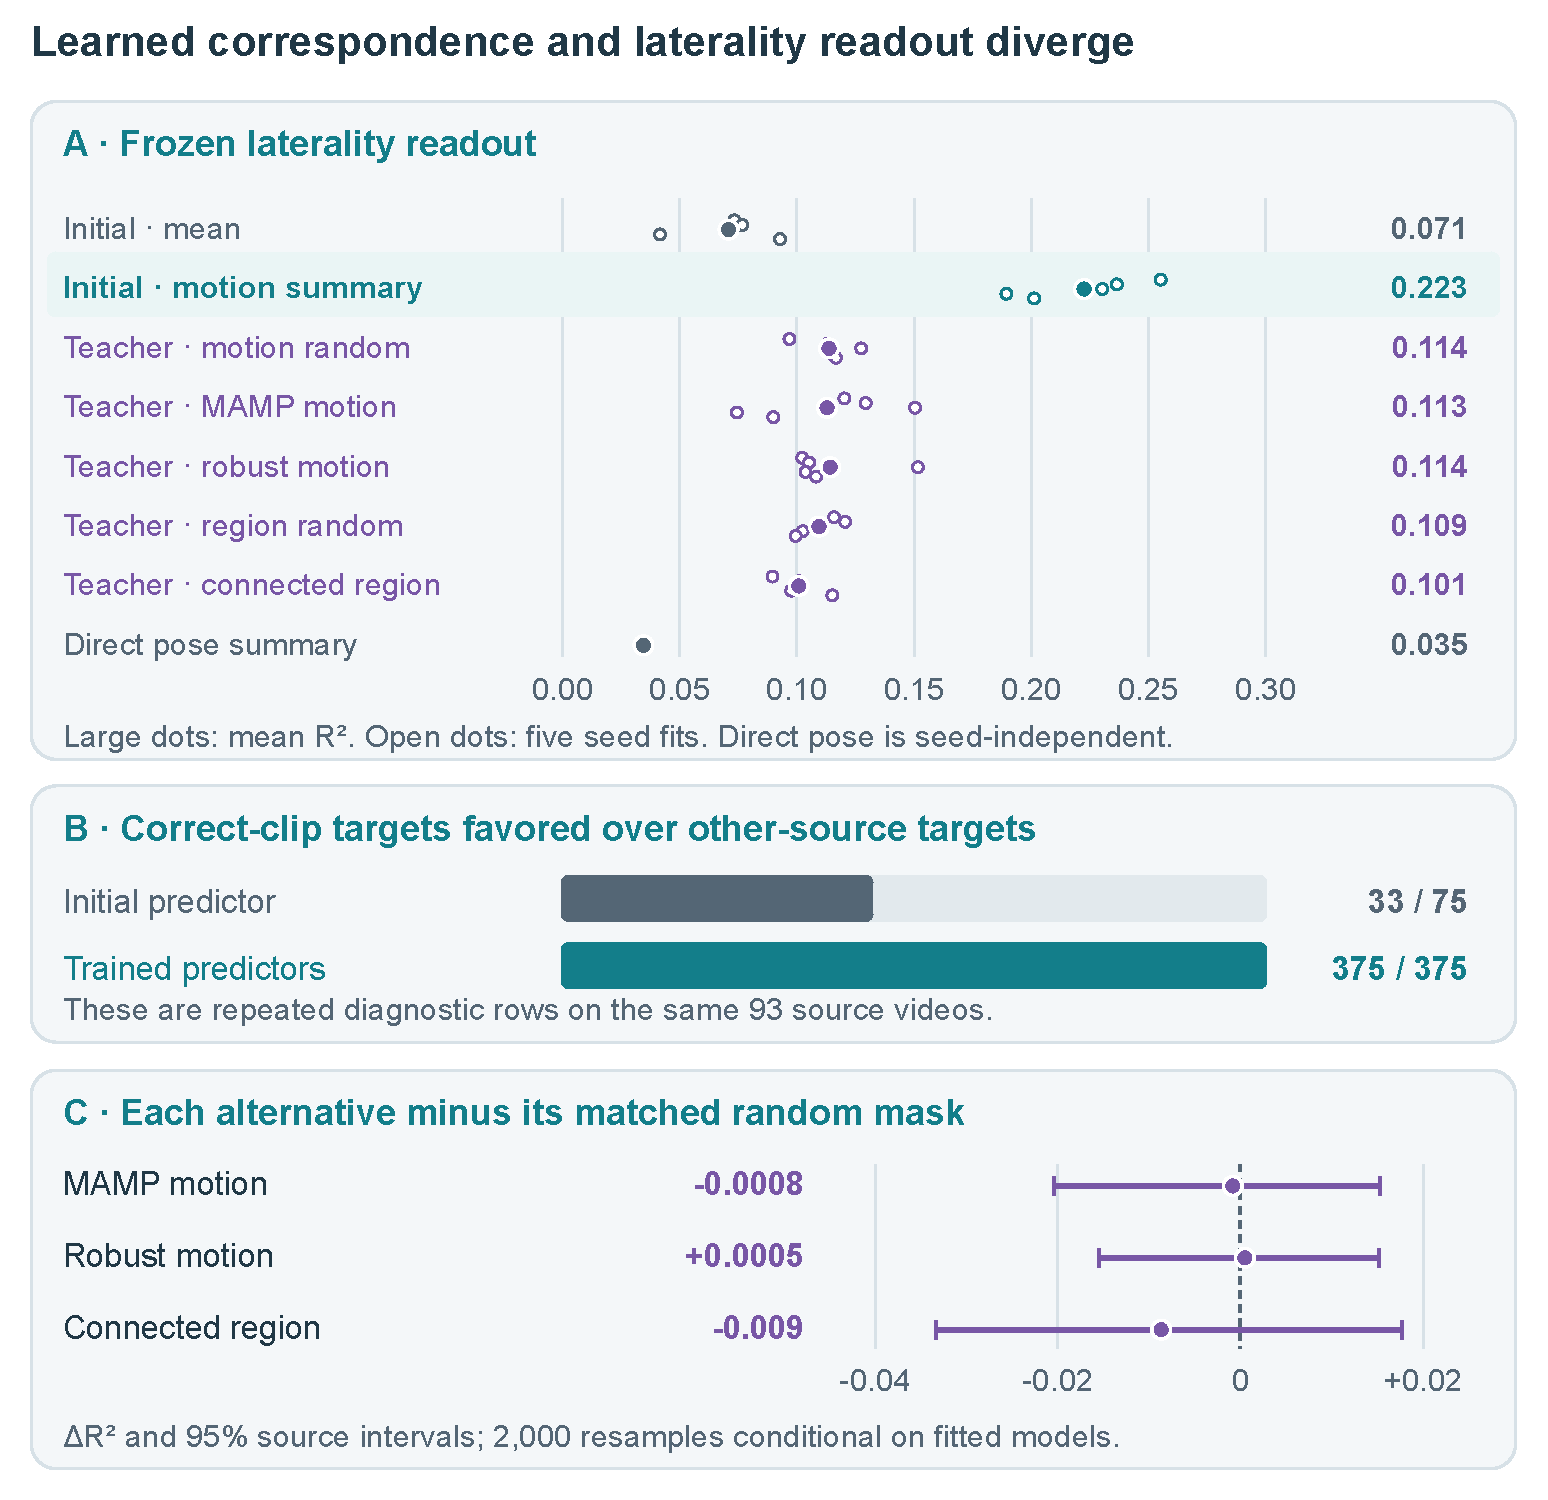
\includegraphics[width=\linewidth]{learning_results_print.pdf}
\caption{Predictors improve clip correspondence while their frozen encoders produce weaker laterality readouts than matched initialization. Seed points are repeated fits on the same 93 videos, not independent cohorts or confidence intervals. The 375 trained diagnostic rows are 125 fits evaluated under three masks; reused initial controls are deduplicated. The Panel C intervals are the retained mask-versus-reference source bootstraps, distinct from Appendix A's new learning contrasts. All plotted values come from the latest saved grid.}\label{fig:learning_results}
\end{figure}

Every trained predictor diagnostic favors its correct clip's hidden teacher features over a valid mismatched target from another source, using the same control clips and positions. Initial controls do not show a consistent preference. Since the teacher features are contextualized using the full clip, this correspondence can depend on information already visible in the context. Static posture, viewpoint, support or motion may contribute; the diagnostic does not isolate recovery of withheld movement.

Each arm predicts its own teacher's feature distributions. A lower loss can accompany changed target variation, so neither raw cross-entropy nor between-arm feature-error magnitudes rank physical usefulness. The shared coordinate-derived endpoint provides the complementary evaluation. Recorded diagnostics do not establish complete feature collapse, and the present results do not identify the mechanism of the learned readout deficit.

\section{Discussion and a decisive next experiment}\label{discussion-and-a-decisive-next-experiment}

The investigation narrows the question at each stage. The known reflection operation supplies a precise measurement relation; prepared-input disagreement limits attribution of an early readout failure. Count-matched masking changes the selected motion and local context, yet produces no demonstrated laterality benefit. A richer readout improves initialization more than trained representations, even while predictors acquire correct-clip correspondence. These findings motivate investigating which parts of the observable movement remain accessible through the entire measurement, representation and readout procedure.

The most economical follow-up uses saved encoders to isolate support fractions, match summary dimensions, expand ridge penalties, and compare target calculations after each preparation step. Appendix B sets out competing explanations and outcomes that would weaken them. A pilot used to choose a pretraining recipe must exclude its validation videos from that encoder's training, not only from its readout fit.

After fixing that evaluation, compare the same recipe with and without explicit reflection training. Success should require improved observable prediction over both the matched base recipe and initialization, the intended transformation behavior, and retained feature variation. A lower \(q\) alone would leave the central utility question open. Measure the extra encoder passes and keep failed outcomes. The current development results can guide that design; a new source collection or independently specified setting is needed for stronger confirmation.

Future prediction would provide a more direct link to temporal world models. Prepare the input from an observed prefix only, predict future teacher features, and decode common future coordinates using a training-fitted decoder. Compare persistence, recent velocity, direct past coordinates, initial encoders and mismatched-future training at identical eligible endpoints. Observed-future features test decoder expressiveness with access to the answer period; they are not a deployable baseline. Appendix C illustrates the current synthetic forecast failure. No real-data forecast or recursive rollout is established here.

\section{Scope, ethics and reproducibility}\label{scope-ethics-and-reproducibility}

The supported scope is post-development, within-GAVD performance on excluded source videos. Repeated people across videos cannot be ruled out. The target has no independent clinical validation, omits temporal phase and loading, and may cancel different pairwise asymmetries. Video-derived coordinates and visibility are one observation pipeline; the study does not demonstrate multimodal sensing, calibrated 3D reconstruction or physiological simulation.

The present review independently reproduces the latest grid's 125,000 prediction rows, 200 pooled score rows and three saved mask intervals, and verifies grid-table hashes and 125 complete update histories. It does not claim to rehash every model checkpoint or reproduce absent historical reports. The {core audit}, {extension audit}, {recomputation script} and {figure provenance} distinguish those evidence levels. Existing research files remain unchanged.

Institutional ethics, data-use and derived-pose release reviews remain unresolved in the governance record. No authorization for submission or artifact release is inferred from public video availability. These revisions are internal manuscript artifacts.
\label{physworld:main-last}
\clearpage
\label{physworld:references-start}
{\renewcommand{\bibfont}{\small}
\begin{thebibliography}{99}
\bibitem{ref01} K. K. Patterson, I. Parafianowicz, C. J. Danells, V. Closson, M. C. Verrier, W. R. Staines, S. E. Black, and W. E. McIlroy. \href{https://pubmed.ncbi.nlm.nih.gov/18226655/}{Gait asymmetry in community-ambulating stroke survivors}. \emph{Archives of Physical Medicine and Rehabilitation}, 89(2):304--310, 2008. doi:10.1016/j.apmr.2007.08.142.

\bibitem{ref02} M. D. Lewek, R. Poole, J. Johnson, O. Halawa, and X. Huang. \href{https://pubmed.ncbi.nlm.nih.gov/19945285/}{Arm swing magnitude and asymmetry during gait in the early stages of Parkinson's disease}. \emph{Gait \& Posture}, 31(2):256--260, 2010. doi:10.1016/j.gaitpost.2009.10.013.

\bibitem{ref03} S. M. Brændvik, T. Goihl, R. S. Braaten, and B. Vereijken. \href{https://pubmed.ncbi.nlm.nih.gov/32082235/}{The Effect of Increased Gait Speed on Asymmetry and Variability in Children With Cerebral Palsy}. \emph{Frontiers in Neurology}, 10:1399, 2020. doi:10.3389/fneur.2019.01399.

\bibitem{ref04} I. Vandekerckhove, M. Van den Hauwe, N. De Beukelaer, E. Stoop, M. Goudriaan, M. Delporte, G. Molenberghs, A. Van Campenhout, L. De Waele, N. Goemans, F. De Groote, and K. Desloovere. \href{https://pmc.ncbi.nlm.nih.gov/articles/PMC9201072/}{Longitudinal Alterations in Gait Features in Growing Children With Duchenne Muscular Dystrophy}. \emph{Frontiers in Human Neuroscience}, 16:861136, 2022. doi:10.3389/fnhum.2022.861136.

\bibitem{ref05} M. Abdelfattah and A. Alahi. \href{https://www.ecva.net/papers/eccv_2024/papers_ECCV/papers/04755.pdf}{S-JEPA: A Joint Embedding Predictive Architecture for Skeletal Action Recognition}. In \emph{Computer Vision -- ECCV 2024}, volume 15090 of \emph{Lecture Notes in Computer Science}, pages 367--384. Springer, 2025. doi:10.1007/978-3-031-73411-3\_21.

\bibitem{ref06} Y. Mao, J. Deng, W. Zhou, Y. Fang, W. Ouyang, and H. Li. \href{https://arxiv.org/abs/2308.07092}{Masked Motion Predictors are Strong 3D Action Representation Learners}. In \emph{Proceedings of the IEEE/CVF International Conference on Computer Vision (ICCV)}, pages 10181--10191, 2023.

\bibitem{ref07} J. Do, Y. Chen, G. Youk, and M. Kim. \href{https://arxiv.org/abs/2603.10648}{Less is More: Compact-Token Masked Feature Prediction for Skeleton Representation Learning}. arXiv preprint arXiv:2603.10648v3, 2026.

\bibitem{ref08} H. Ghaemi, E. B. Muller, and S. Bakhtiari. \href{https://proceedings.neurips.cc/paper_files/paper/2025/hash/2f63d2963526bdd9ff1b8bcc2dc9905a-Abstract-Conference.html}{seq-JEPA: Autoregressive Predictive Learning of Invariant-Equivariant World Models}. In \emph{Advances in Neural Information Processing Systems}, volume 38, pages 32943--32973, 2025. doi:10.52202/085713-1104.

\bibitem{ref09} J. Lee, C. Kim, H. Kim, K. Lee, and J. Lee. \href{https://proceedings.iclr.cc/paper_files/paper/2026/hash/3be6511c8f56d0dca4b5ed59fdf9b2f4-Abstract-Conference.html}{Soft Equivariance Regularization for Invariant Self-Supervised Learning}. In \emph{Proceedings of the International Conference on Learning Representations (ICLR)}, pages 35502--35521, 2026.

\bibitem{ref10} L. Mur-Labadia, M. Muckley, A. Bar, M. Assran, K. Sinha, M. Rabbat, Y. LeCun, N. Ballas, and A. Bardes. \href{https://arxiv.org/abs/2603.14482}{V-JEPA 2.1: Unlocking Dense Features in Video Self-Supervised Learning}. arXiv preprint arXiv:2603.14482v3, 2026.

\bibitem{ref11} H. Wei, L. Sun, and G. Zhao. \href{https://arxiv.org/abs/2608.21160}{Human-JEPA: A Human-Centric Vision Model that Perceives and Anticipates}. arXiv preprint arXiv:2608.21160v1, 2026.

\bibitem{ref12} M. J. Marin-Jimenez, I. Jimenez-Velasco, and R. Muñoz-Salinas. \href{https://github.com/AVAuco/GaitJEPA}{GaitJEPA: How Far Can We Go with JEPA on Binary Silhouettes for Gait Recognition?} Accepted for the \emph{IEEE International Joint Conference on Biometrics (IJCB)}, 2026; author repository, accessed 10 September 2026.

\bibitem{ref13} R. Ranjan, D. Ahmedt-Aristizabal, M. A. Armin, and J. Kim. \href{https://arxiv.org/abs/2407.04190}{Computer Vision for Clinical Gait Analysis: A Gait Abnormality Video Dataset}. \emph{IEEE Access}, 13:45321--45339, 2025. doi:10.1109/ACCESS.2025.3545787.

\bibitem{ref14} Q. Xiong, Y. Liu, J. Mo, Y. Chen, L. Zhang, Z. Xia, C. Yi, S. Jiang, and N. Xiao. \href{https://pmc.ncbi.nlm.nih.gov/articles/PMC10388506/}{Gait asymmetry in children with Duchenne muscular dystrophy: evaluated through kinematic synergies and muscle synergies of lower limbs}. \emph{BioMedical Engineering OnLine}, 22:75, 2023. doi:10.1186/s12938-023-01134-7.

\bibitem{ref15} Google. (2026). \href{https://developers.google.com/edge/mediapipe/solutions/vision/pose_landmarker}{Pose landmark detection guide}. MediaPipe documentation; 33-landmark schema.
\end{thebibliography}
}
\clearpage
\appendix
\label{physworld:appendix-start}
\section{Additional exploratory learning contrasts}\label{appendix-a.-additional-exploratory-learning-contrasts}

These contrasts were calculated during the 9 September revision from the complete latest prediction grid. They were not part of the original registered reflection audit. Each compares the final teacher's motion-sensitive summary with its matched initial encoder using the same readout family, clips and seed. Intervals are marginal percentile source-bootstrap intervals conditional on the fitted models; there is no family-wise multiplicity adjustment.

\begin{table}[htbp]
\centering
\small
\begin{tabular}{@{}
  >{\raggedright\arraybackslash}p{(\linewidth - 4\tabcolsep) * \real{0.4600}}
  >{\raggedleft\arraybackslash}p{(\linewidth - 4\tabcolsep) * \real{0.2200}}
  >{\raggedright\arraybackslash}p{(\linewidth - 4\tabcolsep) * \real{0.3200}}@{}}
\toprule\noalign{}
\begin{minipage}[b]{\linewidth}\raggedright
Training arm
\end{minipage} & \begin{minipage}[b]{\linewidth}\raggedleft
Learned minus initial \(R^2\)
\end{minipage} & \begin{minipage}[b]{\linewidth}\raggedright
95\% source interval
\end{minipage} \\
\midrule\noalign{}

Motion uniform & −0.1088 & {[}−0.1701, −0.0412{]} \\
MAMP-style motion & −0.1097 & {[}−0.1651, −0.0514{]} \\
Robust motion & −0.1083 & {[}−0.1706, −0.0423{]} \\
Region uniform & −0.1131 & {[}−0.1662, −0.0596{]} \\
Connected region & −0.1218 & {[}−0.1828, −0.0553{]} \\
\bottomrule
\end{tabular}
\end{table}

The {recomputation script} checks the prediction coverage and reproduces the recorded pooled scores before calculating these contrasts. The {extension evidence audit} records the retained artifact paths and full-precision values.

\section{Competing explanations and tests that could distinguish them}\label{appendix-b.-competing-explanations-and-tests-that-could-distinguish-them}

\begin{table}[htbp]
\centering
\small
\begin{tabular}{@{}
  >{\raggedright\arraybackslash}p{(\linewidth - 4\tabcolsep) * \real{0.2700}}
  >{\raggedright\arraybackslash}p{(\linewidth - 4\tabcolsep) * \real{0.3800}}
  >{\raggedright\arraybackslash}p{(\linewidth - 4\tabcolsep) * \real{0.3500}}@{}}
\toprule\noalign{}
\begin{minipage}[b]{\linewidth}\raggedright
Explanation compatible with the findings
\end{minipage} & \begin{minipage}[b]{\linewidth}\raggedright
Useful next test
\end{minipage} & \begin{minipage}[b]{\linewidth}\raggedright
Outcome that would weaken it
\end{minipage} \\
\midrule\noalign{}

Preparation changes the relevant measurement & Recompute the target after each preparation stage on common valid transitions, with timestamps retained & Little discrepancy at every stage despite poor learned readouts \\
Summary choice obscures useful features & Compare mean, support-only, temporal SD, increments and their combinations on frozen initial and trained encoders & Deficit persists under adequately selected readouts with matched capacity \\
Ridge regularization is insufficient & Expand the penalty grid identically for all arms using inner training-source validation & Interior selected optima still produce a learned deficit \\
The prescribed reflection action is too restrictive & Fit a shared involutive channel map on training pairs and evaluate held-out pairs, with initial and mismatched controls & No meaningful advantage for genuine reflected pairs on held-out sources \\
Predictive targets emphasize another clip property & Compare local motion supervision or visible-token targets at matched budgets and measure a common observable outcome & Improved internal correspondence still fails to improve the common outcome \\
\bottomrule
\end{tabular}
\end{table}

These are proposed discriminating tests, not explanations established by the current data. Fitting a reflection map that preserves lengths would add an orthogonality assumption; the input reflection does not guarantee that learned feature channels obey it. Any new decision based on this cohort remains development work and should precede confirmation in an independently specified setting.

\section{Geometric and forecasting illustrations}\label{appendix-c.-geometric-and-forecasting-illustrations}

\begin{figure}[!tbp]
\centering
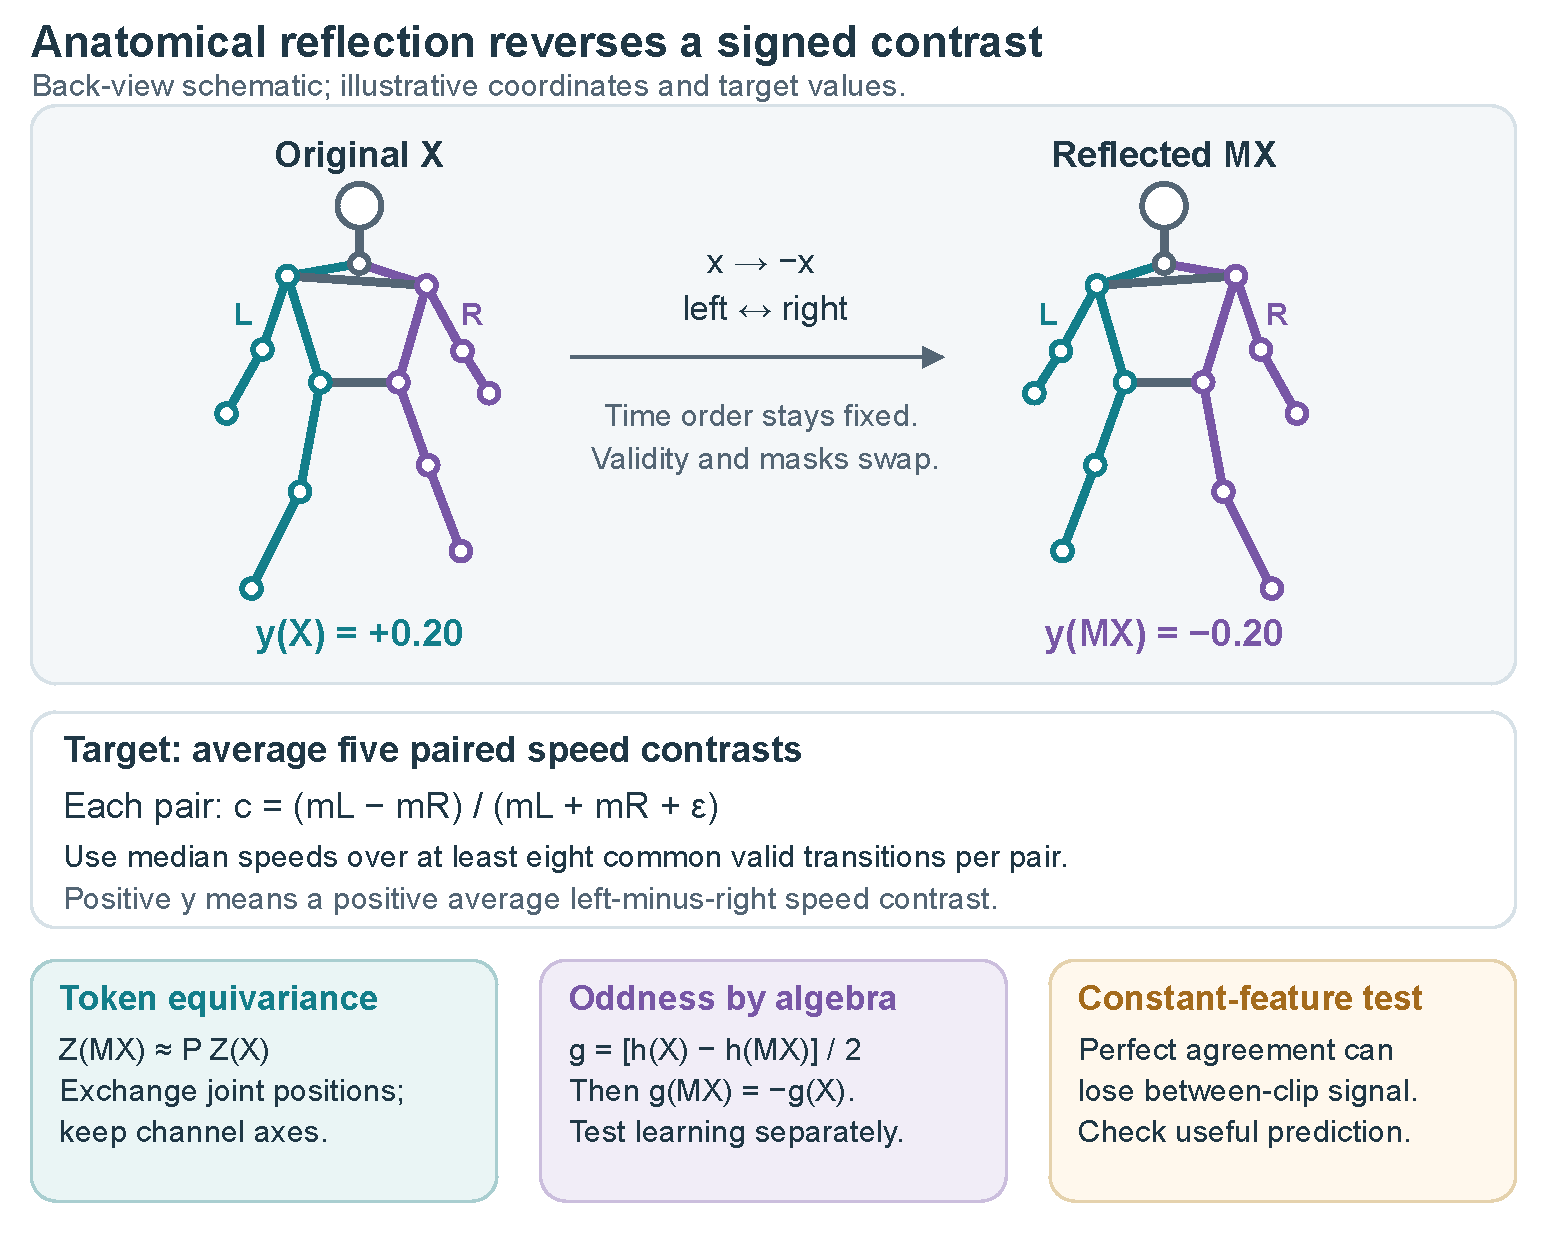
\includegraphics[width=\linewidth]{reflection_and_target_print.pdf}
\caption{Reflection changes the sign of the defined target through horizontal reflection and anatomical exchange. The bodies and values are schematic, not clinical examples. An odd readout can guarantee its output transformation for any encoder. A constant nonzero token representation illustrates why geometric agreement alone is insufficient.}\label{fig:reflection_and_target}
\end{figure}

A simple trajectory construction explains the limits of temporal averaging. Let left positions be \((0,1,0,1)\) and right positions \((0,0,1,1)\) at equal intervals. Both means are 0.5, but median speeds are respectively 1 and 0. Exchanging the trajectories reverses their contrast while retaining the means. This demonstrates a limitation of mean raw positions. An encoder could encode movement before pooling, so it does not prove a limitation of every mean-pooled representation.

Notebook 14's retained synthetic demonstration uses eight generated sources, six for training and two for testing, one seed, and four updates per arm. A decoder fitted on training-source future teacher features is frozen and applied to either observed or predicted future features.

\begin{table}[htbp]
\centering
\small
\begin{tabular}{@{}
  >{\raggedright\arraybackslash}p{(\linewidth - 4\tabcolsep) * \real{0.2000}}
  >{\raggedleft\arraybackslash}p{(\linewidth - 4\tabcolsep) * \real{0.4000}}
  >{\raggedleft\arraybackslash}p{(\linewidth - 4\tabcolsep) * \real{0.4000}}@{}}
\toprule\noalign{}
\begin{minipage}[b]{\linewidth}\raggedright
Future horizon
\end{minipage} & \begin{minipage}[b]{\linewidth}\raggedleft
Observed-future feature RMSE
\end{minipage} & \begin{minipage}[b]{\linewidth}\raggedleft
Predicted-future feature RMSE
\end{minipage} \\
\midrule\noalign{}

0.25 seconds & 0.011 & 2.51 \\
0.50 seconds & 0.013 & 2.61 \\
0.75 seconds & 0.025 & 2.64 \\
\bottomrule
\end{tabular}
\end{table}

These are displayed coordinate RMSE values in normalized coordinate units on 24 common landmark endpoints from two synthetic test clips. They are not calibrated distances. The observed-future route uses information from the answer period and tests decoder expressiveness; the predicted route is the forecast. Its failure after four updates neither establishes real gait performance nor rules out a well-trained forecasting model. Per-example artifacts for this demonstration are absent, so no new uncertainty or finer precision is inferred.

\section{Measurement conventions and information boundaries}\label{appendix-d.-measurement-conventions-and-information-boundaries}

Elapsed time is \((\mathrm{frame\ number}-\mathrm{first\ frame})/\mathrm{fps}\), and speed divides coordinate differences by positive elapsed-time increments. Target normalization uses the observed midpoint of both hips at each frame. If either hip is unavailable, that frame cannot support the target. The scale is the median of valid shoulder-pair and hip-pair widths across the clip; the implementation uses 1 when a usable scale is absent or degenerate. The target contrast uses \(\epsilon=10^{-8}\).

Input normalization separately permits a median pelvis fallback, or zero when no pelvis is observed, after short-gap interpolation. It resizes values and validity to 64 positions; validity must reach 0.999 after resizing, and invalid input values are zeroed. These are engineering conventions for noisy pose estimates, rather than a recovery of anatomical metric geometry. For past-only tasks, all such references must be estimated from the permitted prefix.

Reported prepared-coordinate corruption tests remove only small gaps after normalization and interpolation. Previously removed observations can already have influenced those operations. Those results concern representation sensitivity, not performance under genuinely absent raw observations, and are excluded from the main efficacy argument.

\section{Annotation census and clinical motivation}\label{appendix-e.-annotation-census-and-clinical-motivation}

\begin{table}[htbp]
\centering
\small
\begin{tabular}{@{}
  >{\raggedright\arraybackslash}p{(\linewidth - 4\tabcolsep) * \real{0.1800}}
  >{\raggedleft\arraybackslash}p{(\linewidth - 4\tabcolsep) * \real{0.1700}}
  >{\raggedright\arraybackslash}p{(\linewidth - 4\tabcolsep) * \real{0.6500}}@{}}
\toprule\noalign{}
\begin{minipage}[b]{\linewidth}\raggedright
Local annotation
\end{minipage} & \begin{minipage}[b]{\linewidth}\raggedleft
Clips / sources
\end{minipage} & \begin{minipage}[b]{\linewidth}\raggedright
Relevant published observation and implication
\end{minipage} \\
\midrule\noalign{}

Normal & 270 / 29 & Supplies the dataset reference category; a zero signed contrast is not a clinical definition of normal walking. \\
Stroke & 75 / 18 & Spatial and temporal asymmetries differ across walkers; a single speed contrast covers only part of gait behavior. Patterson et al.~\citep{ref01} \\
Parkinson's & 39 / 9 & Arm-swing asymmetry motivates preserving side identity; our shoulder points do not measure arm swing directly. Lewek et al.~\citep{ref02} \\
Cerebral palsy & 58 / 9 & Studies include unilateral and bilateral presentations and examine speed-dependent symmetry. Gait-speed study~\citep{ref03} \\
Myopathic & 183 / 28 & Dystrophy studies examine pelvic compensation and multisegment asymmetry, illustrating features beyond this target. Longitudinal kinematics~\citep{ref04}, kinematic-synergy study~\citep{ref14} \\
\bottomrule
\end{tabular}
\end{table}

These are literature-based motivations, not findings about clinical differences in our cohort. In particular, the broad myopathic annotation does not identify Duchenne muscular dystrophy. The data do not supply verified affected-side labels, standardized disease severity, or the subtype information needed to connect target sign to a particular impairment. Here, laterality means a signed comparison of estimated left- and right-side movement.

\section{Training details and explicit geometric supervision}\label{appendix-f.-training-details-and-explicit-geometric-supervision}

The latest recipe uses AdamW with learning rate \(10^{-3}\), weight decay 0.05, gradient clipping at 1, teacher EMA 0.999, student/teacher temperatures 0.10/0.06 and target-center EMA 0.9. CUDA BF16 computation retains FP32 weights, loss reductions and frozen evaluation. The original .6 gait-token mask and later .5 motion budget differ; neither is a fraction of the entire input. Valid region masks use six connected landmarks across eight time blocks, with equal realized counts in their paired reference. Equal updates do not establish equal runtime.

For clip \(b\), define \(D_b=\|Z_\theta(Mx_b)-S Z_\theta(x_b)\|_{C_b}^2\) and \(E_b=\|Z_\theta(Mx_b)\|_{C_b}^2+\|S Z_\theta(x_b)\|_{C_b}^2\), where \(C_b\) identifies common valid positions. Notebook 09 adds \[
\mathcal L_{\mathrm{refl}}=\frac1B\sum_b
\frac{D_b}{\max(\operatorname{stopgrad}(E_b),10^{-12})}.
\] This matches the implementation's detached, clamped denominator. Both numerator branches update the shared online encoder through two additional unmasked passes. The demonstration uses weight 1, 16 input frames and width 16. It has no real-GAVD result and supplies no signed target supervision. Identity action on feature channels is a modeling choice; a constant nonzero representation can satisfy it.

The expanded pipeline (Figure~\ref{fig:training_pipeline}) and {figure documentation} explain all training and evaluation entry points. For the proposed extension, a fitted involutive feature-channel action or explicit even/odd channels would test another geometric assumption. Neither has a completed real-data result in this package.

\section{Historical results retained as context}\label{appendix-g.-historical-results-retained-as-context}

The original figure JSON supplies three-decimal values, while the existing docs README retains five-decimal historical estimates and a claim of prior artifact verification. That prior verification cannot be repeated from the current checkout because the original report/prediction/checkpoint chain is absent. No unavailable value is inferred.

\begin{table}[htbp]
\centering
\small
\begin{tabular}{@{}
  >{\raggedright\arraybackslash}p{(\linewidth - 4\tabcolsep) * \real{0.4600}}
  >{\raggedleft\arraybackslash}p{(\linewidth - 4\tabcolsep) * \real{0.2200}}
  >{\raggedright\arraybackslash}p{(\linewidth - 4\tabcolsep) * \real{0.3200}}@{}}
\toprule\noalign{}
\begin{minipage}[b]{\linewidth}\raggedright
Historical comparison
\end{minipage} & \begin{minipage}[b]{\linewidth}\raggedleft
Estimate
\end{minipage} & \begin{minipage}[b]{\linewidth}\raggedright
Recorded 95\% interval
\end{minipage} \\
\midrule\noalign{}

Learned primary \(R^2\) & 0.05979 & {[}−0.02527, 0.12571{]} \\
Learned minus initial \(R^2\) & −0.01798 & {[}−0.03851, 0.00248{]} \\
Reflection augmented minus vanilla \(R^2\) & 0.00408 & {[}−0.00556, 0.01277{]} \\
Reflection augmented minus vanilla token \(q\) & −0.00843 & {[}−0.01020, −0.00687{]} \\
Learned minus initial token \(q\), vanilla & 0.03055 & {[}0.01576, 0.04763{]} \\
Learned constructed-odd \(R^2\) & 0.04302 & {[}−0.04356, 0.11283{]} \\
Learned minus initial constructed-odd \(R^2\) & −0.05874 & {[}−0.09549, −0.01740{]} \\
\bottomrule
\end{tabular}
\end{table}

The token test uses \(q=D/E\) after joint permutation with identity channel action. Learned vanilla \(q=0.114\), interval {[}0.095,0.138{]}, is retained at three decimals; its interval crosses the operational 0.10 margin, while failing the upper-bound acceptance rule. A low q can reflect insensitive shared features.

The odd construction uses \(z^-(x)=[z(x)-z(Mx)]/\sqrt2\), no feature centering and no readout intercept. Its sign reversal is algebraic. The reported performance tests the whole readout pipeline and cannot identify every source of its useful information.

Notebook 12's retained teacher \(R^2\) values are −0.022633 for gait targets and −0.010449 for all-landmark targets, with initial 0.048160 and direct pose 0.129978. The all-landmark-minus-gait contrast is 0.012184, interval {[}−0.018303,0.050207{]}. Its raw predictions were unavailable for this review. Notebook 08 used an earlier implementation and fixed penalty; its more negative numbers are omitted from the main argument. Comparing scores across these recipes cannot isolate a masking or regularization effect.

\section{Latest absolute results and notebook map}\label{appendix-h.-latest-absolute-results-and-notebook-map}

\begin{table}[htbp]
\centering
\small
\begin{tabular}{@{}
  >{\raggedright\arraybackslash}p{(\linewidth - 4\tabcolsep) * \real{0.4700}}
  >{\raggedleft\arraybackslash}p{(\linewidth - 4\tabcolsep) * \real{0.2900}}
  >{\raggedleft\arraybackslash}p{(\linewidth - 4\tabcolsep) * \real{0.2400}}@{}}
\toprule\noalign{}
\begin{minipage}[b]{\linewidth}\raggedright
Frozen features or control
\end{minipage} & \begin{minipage}[b]{\linewidth}\raggedleft
Mean \(R^2\) ± seed SD
\end{minipage} & \begin{minipage}[b]{\linewidth}\raggedleft
Mean absolute error
\end{minipage} \\
\midrule\noalign{}

Training-source target mean & −0.0106 ± 0.0000 & 0.046172 \\
Direct prepared-pose summary & 0.0345 ± 0.0000 & 0.044960 \\
Initial encoder, mean summary & 0.0708 ± 0.0186 & 0.044344 \\
Initial encoder, motion-sensitive summary & 0.2225 ± 0.0268 & 0.041546 \\
Motion-uniform teacher, motion-sensitive & 0.1137 ± 0.0110 & 0.043658 \\
MAMP-style teacher, motion-sensitive & 0.1129 ± 0.0306 & 0.043751 \\
Robust-motion teacher, motion-sensitive & 0.1142 ± 0.0210 & 0.043595 \\
Region-uniform teacher, motion-sensitive & 0.1094 ± 0.0088 & 0.044037 \\
Connected-region teacher, motion-sensitive & 0.1008 ± 0.0092 & 0.043756 \\
\bottomrule
\end{tabular}
\end{table}

Each row covers 625 clips and 93 sources. SD describes the five optimization seeds, not sampling uncertainty. The initial encoder, direct-pose, and training-mean controls are reused across arms; their repeated appearance in machine-readable tables is not independent replication. ``Initial'' refers only to the S-JEPA weights: the pipeline still uses a pretrained pose detector, supplied anatomical identities, feature engineering, and a supervised ridge readout.

\begin{table}[htbp]
\centering
\small
\begin{tabular}{@{}
  >{\raggedright\arraybackslash}p{(\linewidth - 4\tabcolsep) * \real{0.1300}}
  >{\raggedright\arraybackslash}p{(\linewidth - 4\tabcolsep) * \real{0.4000}}
  >{\raggedright\arraybackslash}p{(\linewidth - 4\tabcolsep) * \real{0.4700}}@{}}
\toprule\noalign{}
\begin{minipage}[b]{\linewidth}\raggedright
Notebooks
\end{minipage} & \begin{minipage}[b]{\linewidth}\raggedright
Question or role
\end{minipage} & \begin{minipage}[b]{\linewidth}\raggedright
Evidence used here
\end{minipage} \\
\midrule\noalign{}

00--02 & Protocol, target/cohort audit and source splits & Code, cohort and splits checked; current scope is internally fixed after development \\
03--05 & Fold-local training, held-out probes and aggregation & Historical summary; original complete report chain unavailable \\
06 & External-subject evaluation gate & No completed external validation \\
07 & Measurement and readout diagnostics & Prepared-target agreement recomputed on 623 clips / 92 sources \\
08 & Earlier matched-count anatomical masking & Historical context; not pooled with later recipes \\
09 & Explicit reflection training & Synthetic only \\
10 & Past-only movement prediction & Implemented route; no retained real training result \\
11--13 & Mask construction, controlled training and predictor/readout checks & Notebook 12 retained real summaries; teaching executions separately synthetic \\
14 & Decode observed versus predicted future features & Synthetic demonstration only \\
15--16 & Motion selection and structured-context audits & Real-data intervention checks \\
17--18 & Paired training and motion-sensitive readouts & Complete latest grid independently recomputed \\
\bottomrule
\end{tabular}
\end{table}
\clearpage
\section{Expanded training pipeline}
\begin{figure}[htbp]
\centering
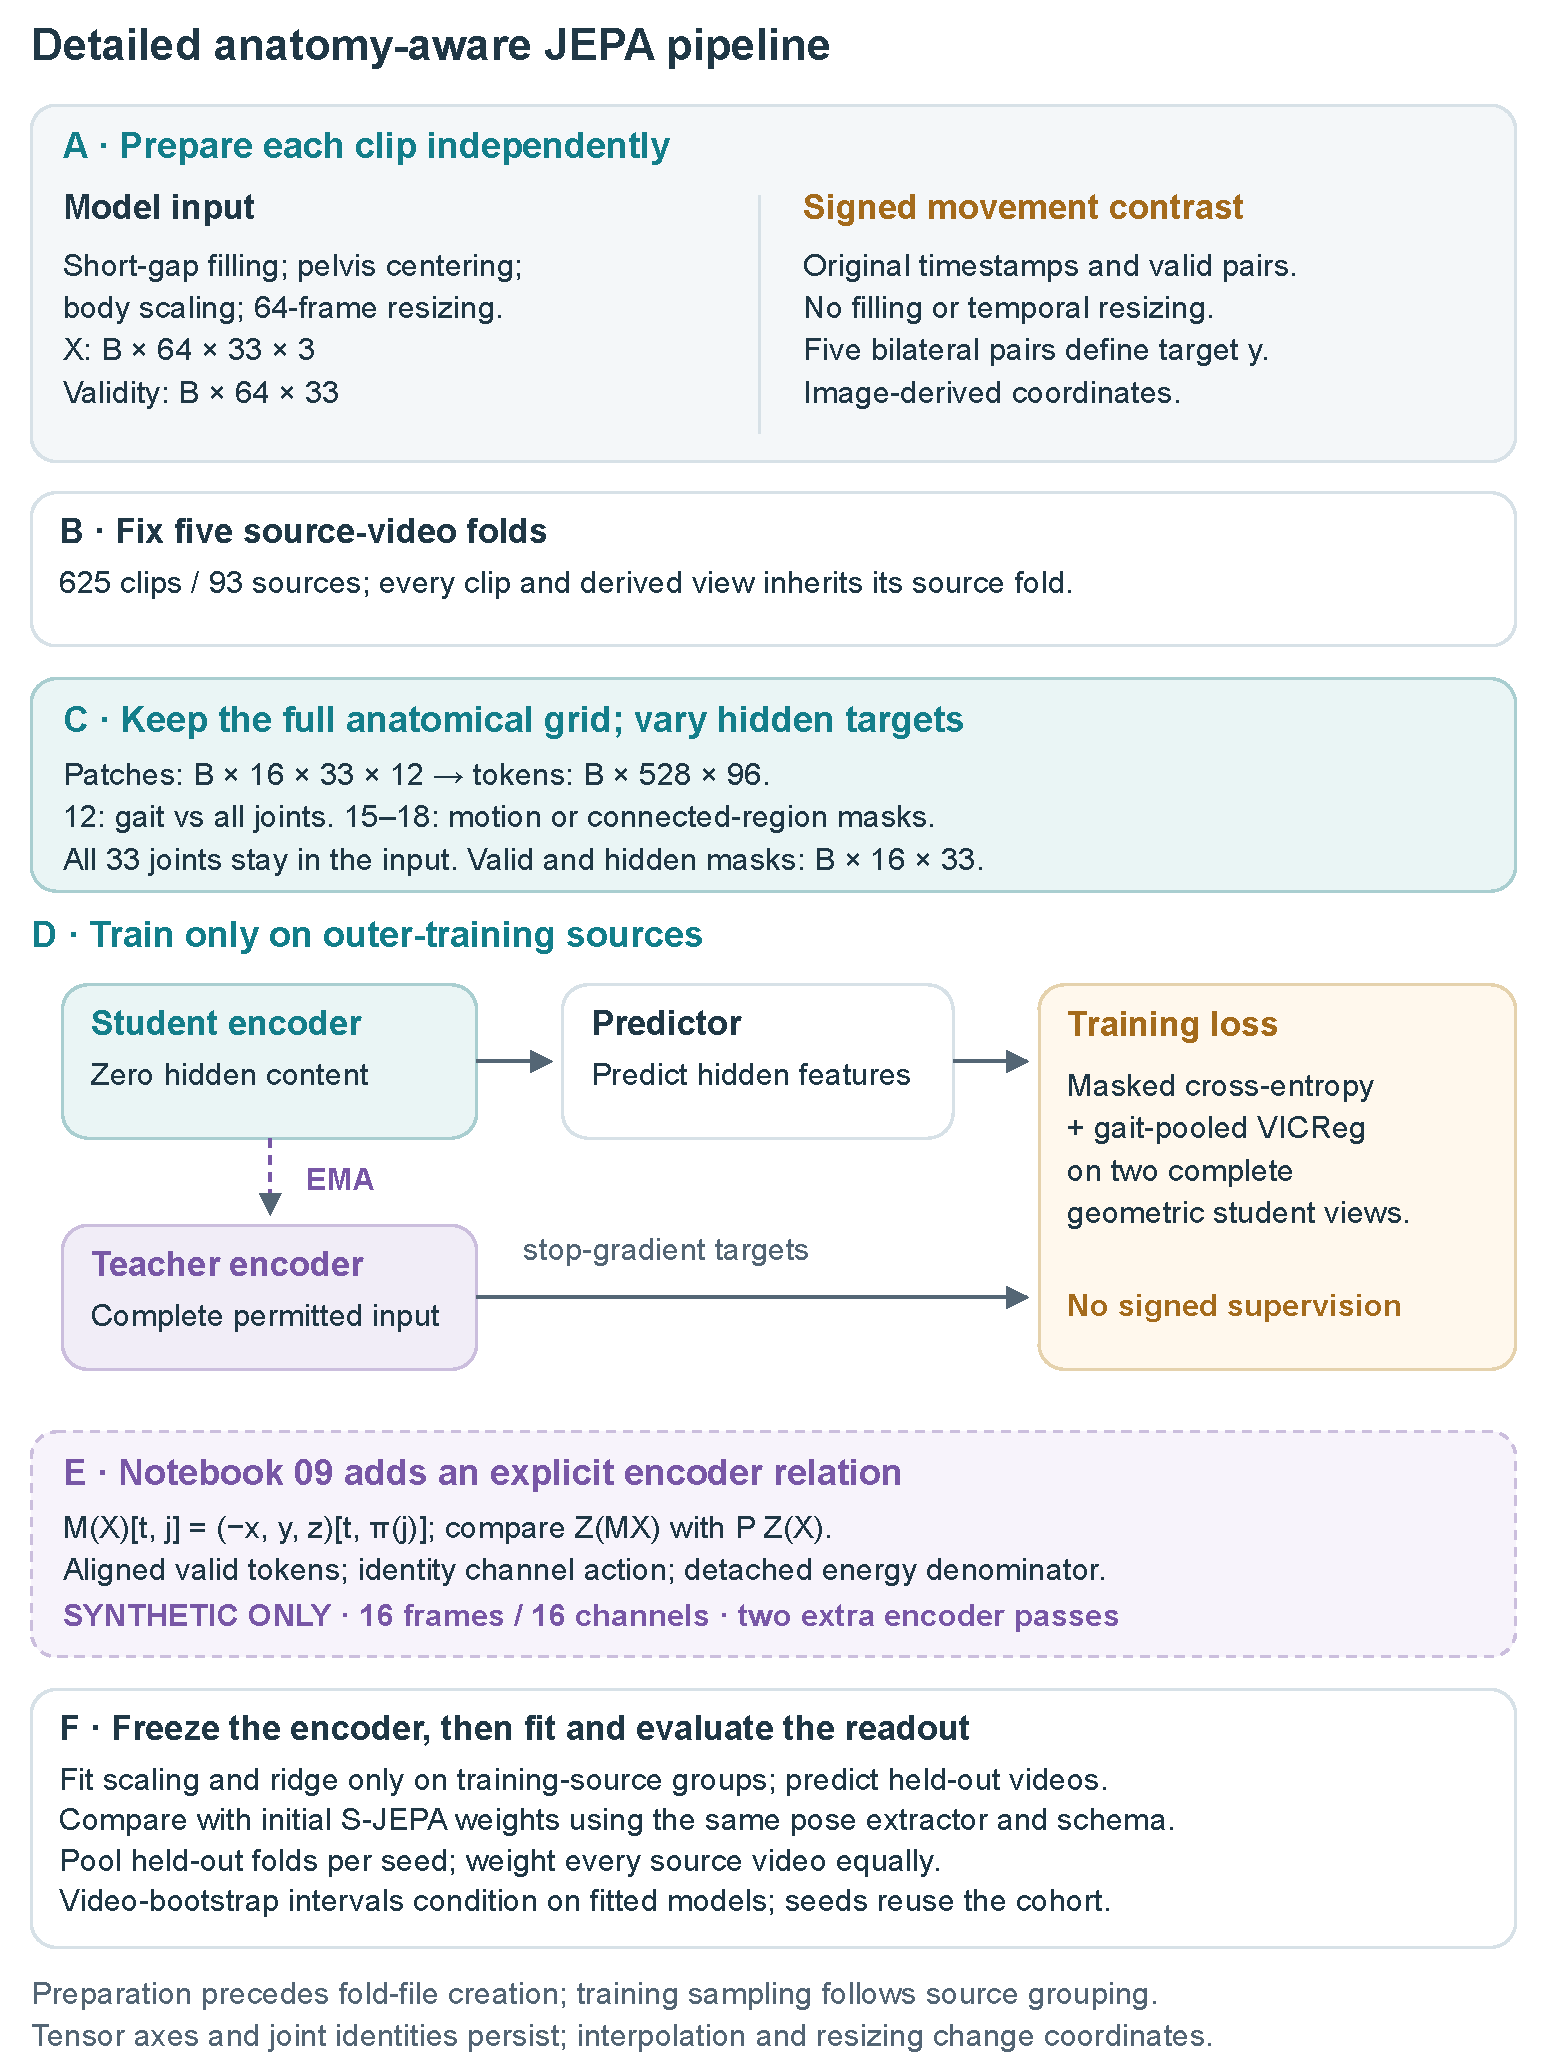
\includegraphics[width=\linewidth]{training_pipeline_print.pdf}
\caption{Expanded version of the training pipeline linked in Figure 1, showing tensor shapes, source separation, and the distinct gradient paths for the completed training recipe and the synthetic reflection extension.}\label{fig:training_pipeline}
\end{figure}

\clearpage
\section{Anatomical selections and input shape}
\begin{figure}[htbp]
\centering
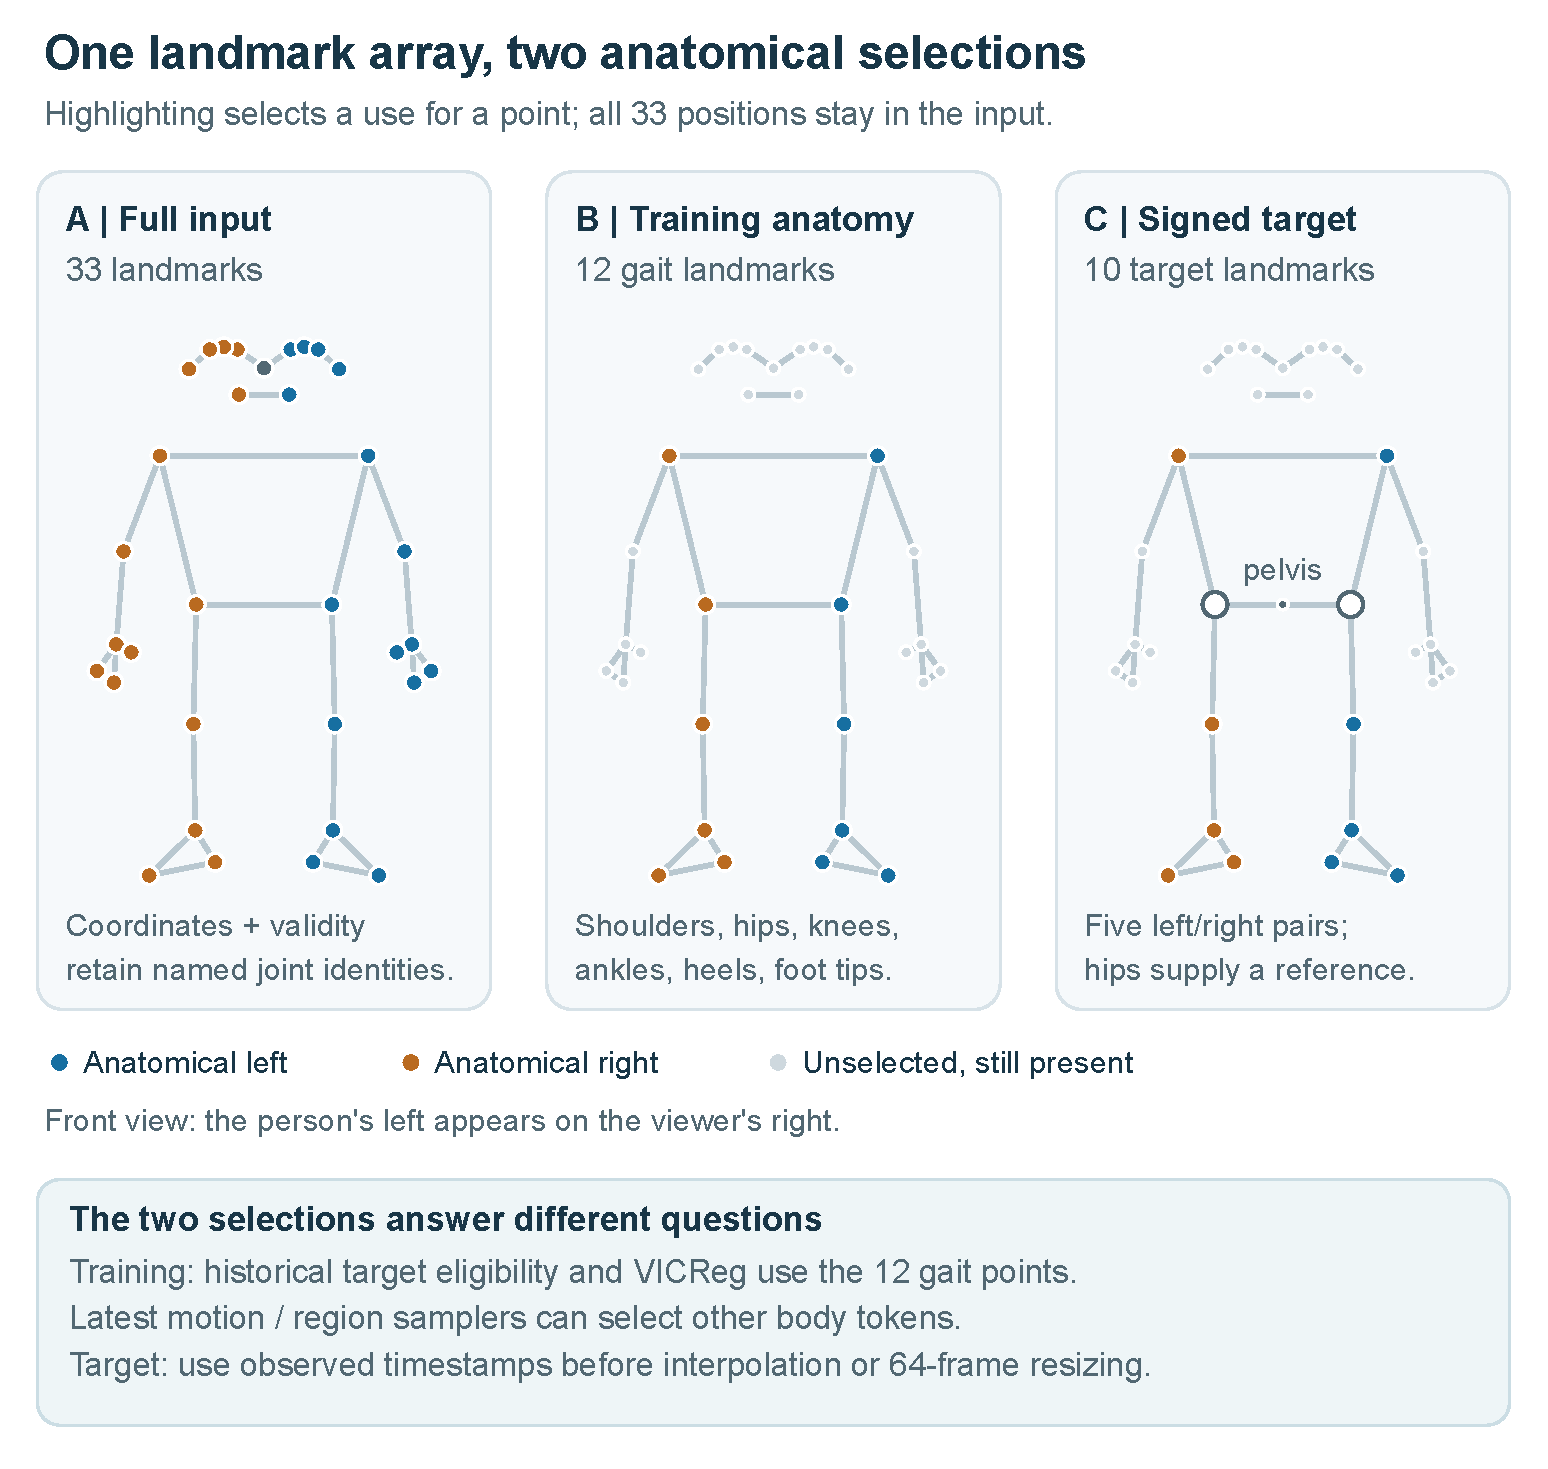
\includegraphics[width=\linewidth]{pose_landmarks_and_laterality.pdf}
\caption{Landmark-selection schematic using the published MediaPipe identities~\citep{ref15}. All 33 positions remain allocated in the encoder input. The 12 highlighted gait landmarks identify historical target eligibility and VICReg pooling; the latest motion and region samplers can select other tokens. The signed target uses five bilateral pairs, with hips supplying the pelvis reference rather than a sixth contrast. Coordinates are hand-drawn for explanation and represent neither measured trajectories nor disease examples.}
\label{fig:pose_landmarks_and_laterality}
\end{figure}

\end{document}
